\section{模型与方法}\label{sec:methods}

\subsection{器件与 Lugiato--Lefever 模型}\label{sec:lle}

我们考虑一个石英微腔：自由光谱范围（FSR）$200~\mathrm{GHz}$，有效群折射率 $1.45$（导模的假设值），往返长度 $L\approx1.03~\mathrm{mm}$，
非线性系数 $\gamma=0.016~\mathrm{W^{-1}m^{-1}}$，群速度色散 $\beta_2=-4\times10^{-27}~\mathrm{s^2/m}$（反常色散），泵浦波长 $1550~\mathrm{nm}$；
这些是代表性数值，不对应某个已制备的器件。
微环有一个输入（直通）端口和一个下载（drop）端口，本征品质因数 $\Qint=10^{8}$；
输入端口的耦合品质因数 $\Qone$ 是每个工作点的随机参数，取值 $10^{5.8}$ 到 $10^{7.2}$，
下载端口的耦合品质因数默认为 $\Qtwo=2.2\times10^{7}$（第~\ref{sec:readout}~节的“加大下载端口耦合”变体在 $10^{6}$ 到 $2.2\times10^{7}$ 之间取）。
总品质因数在 $6\times10^{5}$ 到 $8\times10^{6}$ 之间（加大下载端口耦合时可低到 $4\times10^{5}$），对应的半线宽约 $12$ 到 $160~\mathrm{MHz}$（$250~\mathrm{MHz}$），
光子寿命约 $0.5$ 到 $7~\mathrm{ns}$（$0.3~\mathrm{ns}$），与符号时间同一量级。从下载端口读出，是为了让探测到的光经过谐振滤波，不被未耗尽的输入泵浦主导。
图~\ref{fig:scheme}a 是整个方案的光路，图~\ref{fig:scheme}b 是本节建立的仿真模型：从输入掩模、腔内动力学、下载端口、探测到线性读出，以及各项噪声进入的位置。

\begin{figure}[htbp]
\centering
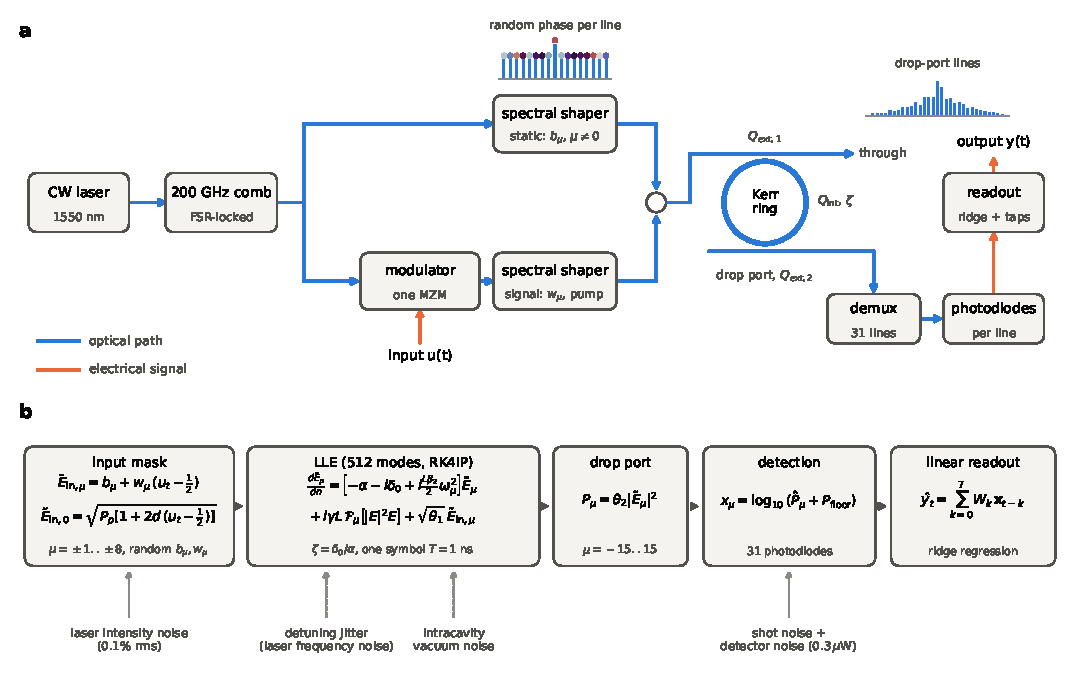
\includegraphics[width=\linewidth]{fig1_scheme}
\caption{方案与模型。
（a）光路：与微环自由光谱范围锁定的 $200~\mathrm{GHz}$ 输入光梳分成两路，静态的一路经谱整形器写入偏置 $b_\mu$ 并挡掉中心（泵浦）梳齿，
另一路经一个调制器承载信号 $u(t)$、再经谱整形器写入权重 $w_\mu$ 并放过泵浦，所以泵浦功率按式~\eqref{eq:mask} 被调制；
两路合束后送入加载--下载型 Kerr 微腔（输入耦合 $\Qone$、下载耦合 $\Qtwo$、本征 $\Qint$、归一化失谐 $\zeta$）。
下载端口的 31 根梳齿经解复用后分别探测，由带延迟抽头的岭回归读出层组合成输出 $y(t)$。插图：输入梳齿的随机相位（颜色）和下载端口光谱的示意。
（b）仿真模型的信号流：输入掩模（式~\eqref{eq:mask}）、Lugiato--Lefever 方程（式~\eqref{eq:lle}）、下载端口功率、对数探测和线性读出；
虚线箭头标出五项噪声进入的位置（第~\ref{sec:noise-model}~节）。}
\label{fig:scheme}
\end{figure}

腔内场用平均场的 Lugiato--Lefever 方程（LLE）描述~\cite{lugiato1987,coen2013}。
以往返次数 $n=t/t_R$ 为慢时间，记第 $\mu$ 个纵模（相对泵浦）的场振幅为 $\tilde E_\mu$，其角频率偏移为 $\omega_\mu=2\pi\,\mathrm{FSR}\,\mu$，则
\begin{equation}
\frac{\mathrm d\tilde E_\mu}{\mathrm dn}
=\Big[-\alpha-i\delta_0+i\frac{L\beta_2}{2}\,\omega_\mu^{2}\Big]\tilde E_\mu
+i\gamma L\,\mathcal F_\mu\!\big[|E|^{2}E\big]
+\sqrt{\theta_1}\,\tilde E_{\mathrm{in},\mu}(u_t),
\label{eq:lle}
\end{equation}
其中 $t_R=1/\mathrm{FSR}$ 是往返时间，$E(\tau)$ 是快时间网格上的腔内场（$|E|^2$ 以瓦为单位），$\mathcal F_\mu$ 表示取第 $\mu$ 个傅里叶分量
（约定 $E(\tau)=\sum_\mu\tilde E_\mu e^{-i\omega_\mu\tau}$），$\alpha_i$ 是每往返一次的本征功率损耗，
$\theta_1$、$\theta_2$ 是两个端口的功率耦合率，$\alpha=(\alpha_i+\theta_1+\theta_2)/2$ 是每往返一次的场衰减（半线宽），
$\delta_0$ 是泵浦相对谐振的失谐。下文用归一化失谐 $\zeta=\delta_0/\alpha$（以半线宽为单位）。
总品质因数与衰减的关系为 $Q=\omega_0 t_R/(2\alpha)$。
下载端口第 $\mu$ 根梳齿的光功率为 $P_\mu=\theta_2|\tilde E_\mu|^{2}$。

方程~\eqref{eq:lle} 用相互作用绘景下的四阶龙格--库塔法（RK4IP）~\cite{hult2007} 积分，只由快速傅里叶变换和逐点运算构成，
因此可以对所有器件参数求梯度（第~\ref{sec:gradient}~节）。
默认用 512 个纵模，每个 $1~\mathrm{ns}$ 的符号（约 200 次往返）积分 20 步。
我们检查了网格收敛：主结果在 512 与 1024 个模式之间一致，早先观察到的约 30\% 差别来自选点时的乐观偏差，而不是网格（补充材料）。

\subsection{输入编码}\label{sec:encodings-def}

输入信号是一串符号 $u_t\in[0,1]$，每个符号持续 $T=1~\mathrm{ns}$，期间输入场保持不变。
我们比较八种把 $u_t$ 送进微环的方式。

\paragraph{谱相位输入掩模（本文）。}
输入场由泵浦（$\mu=0$）和两侧各 8 根输入梳齿（$\mu=\pm1,\dots,\pm8$）组成：
\begin{equation}
\tilde E_{\mathrm{in},0}=\sqrt{P_p\,[1+2d\,(u_t-\tfrac12)]},\qquad
\tilde E_{\mathrm{in},\mu}=b_\mu+w_\mu\,(u_t-\tfrac12)\quad(\mu=\pm1,\dots,\pm8).
\label{eq:mask}
\end{equation}
每根梳齿的偏置 $b_\mu$ 和调制权重 $w_\mu$ 是独立抽取的复高斯数，即随机的幅度和随机的相位；
它们整体缩放，使边带的平均功率 $\sum_\mu\big(|b_\mu|^{2}+|w_\mu|^{2}/12\big)$ 等于总功率 $P$ 的一个比例 $f_s$，泵浦功率 $P_p=(1-f_s)P$。
每个工作点的随机参数是总功率 $P$（$10$ 到 $300~\mathrm{mW}$，对数均匀）、$f_s\in[0.1,0.9]$、调制深度 $d\in[0.05,0.9]$、$\zeta\in[-1,4]$ 和 $\Qone$。
在实验上，这相当于把一个输入光梳分成两路，一路保持静止（给出 $b_\mu$），一路经过一个调制器（给出 $w_\mu$），
两路各经过一个可编程的谱整形器后再合束。第~\ref{sec:ablation}~节的消融显示，真正起作用的是各梳齿相位的随机性，
所以谱整形器只需要设定相位。

\paragraph{单泵浦编码（我们对文献方案的实现）。}
只用一个连续泵浦，信号调制它的功率 $P[1+d(u_t-\tfrac12)]$、失谐 $\zeta+d(u_t-\tfrac12)$ 或相位 $\exp[i d(u_t-\tfrac12)]$，
分别参照文献~\cite{shishavan2025}、\cite{cuevas2025}、\cite{arabieh2026soliton}。这些是放在统一器件和协议下的实现，不是对原文装置的复现
（原文没有给全腔长、$Q$ 分配和采样间隔）。三种编码各有两组。从零场起振时，$\zeta\in[-1,4]$、$P\in[10,300]~\mathrm{mW}$ 与掩模相同，
功率编码 $d\in[0.05,1]$，失谐和相位编码的 $d$ 在 $[10^{-1.3},10^{0.5}]$ 内对数均匀抽取。
从单孤子出发时，$\Qone\in[10^{6.5},10^{7.2}]$、$P\in[30,300]~\mathrm{mW}$，$\zeta$ 在孤子存在区间内（从 2 到其上限）抽取，
功率编码 $d\in[0.02,0.5]$，失谐编码 $d$ 在 $[10^{-1.3},10^{0}]$、相位编码在 $[10^{-1.3},10^{0.5}]$ 内对数均匀抽取。

\paragraph{整体调制的光梳。}
与掩模相同的 16 根输入梳齿，但幅度相同、相位相同，所有梳齿一起被同一个信号调制，相当于一串被调制的同步脉冲~\cite{arabieh2026pulse}。

所有编码使用相同的器件、相同的功率和 $Q$ 范围、相同的读出，并且各抽相同数量的随机工作点（第~\ref{sec:protocol}~节）。

\subsection{读出}\label{sec:readout-def}

下载端口的中心 31 根梳齿（$\mu=-15,\dots,15$）经解复用后由光电探测器分别探测。
读数取对数，$x_\mu=\log_{10}(\hat P_\mu+P_\mathrm{floor})$，其中 $\hat P_\mu$ 是带噪声的读数，
$P_\mathrm{floor}$ 取探测器噪声与 $1~\mathrm{nW}$ 中较大者，避免没有光的梳齿在取对数后主导回归。
读出层除了当前符号的 31 个读数，还看前 7 个符号的读数（8 个延迟抽头，共 248 个特征；NARMA-10 用 12 个抽头），
用带标准化的岭回归，正则化强度在 $\{10^{-8},10^{-6},10^{-4},10^{-2},1\}$ 中按验证误差选取。
第~\ref{sec:memory}~节专门讨论这些抽头带来的记忆。

\subsection{噪声模型}\label{sec:noise-model}

“现实噪声”包括器件内的三项和探测端的两项：
\begin{itemize}
\item 激光强度噪声：相对均方根 $0.1\%$，每个符号一个样本，泵浦和所有输入梳齿共用；
\item 失谐抖动：泵浦相对谐振的失谐每个符号抖动半线宽的 $1\%$（均方根），为一阶自回归过程，相邻符号的相关系数为 $e^{-1}$。
      因为它按线宽的比例定义，等效的激光线宽随 $Q$ 变化（式~\eqref{eq:linewidth}）：$Q=1.9\times10^{6}$ 时约 $1.6~\mathrm{kHz}$，$Q=6\times10^{6}$ 时只有约 $160~\mathrm{Hz}$。
      所以随机搜索对高 $Q$ 点的惩罚比固定的激光轻；第~\ref{sec:laser}~节对最好的单环改用绝对的激光频率噪声谱，在固定激光下的全面重选留作后续工作；
\item 腔内场噪声：真空涨落水平，每个损耗通道每个模式半个光子；
\item 散粒噪声：每个读数积分一个符号时间（$1~\mathrm{ns}$）；
\item 探测器电子噪声：每根梳齿 $0.3~\mu\mathrm{W}$（折合到光功率的均方根）。
      1~GHz 量级的 InGaAs PIN 接收机，按手册的等效噪声功率折算为每根梳齿 $0.13$ 到 $0.63~\mu\mathrm{W}$，$0.3~\mu\mathrm{W}$ 居中。
\end{itemize}
放大器自发辐射的自拍频噪声和探测器量子效率没有建模。第~\ref{sec:noise}~节逐项拆分这些噪声的贡献。

\subsection{任务与软件基线}\label{sec:tasks}

三个基准任务：
（1）Mackey--Glass 时间序列~\cite{mackey1977}（延迟 17，反馈率 0.2、衰减率 0.1，指数 10，采样间隔 1）的 10 步预测；
（2）非线性信道均衡~\cite{jaeger2004}：四电平符号经过线性符号间干扰、三阶多项式非线性和信噪比 $28~\mathrm{dB}$ 的加性噪声，
从接收信号恢复两个符号之前发送的符号，除 NMSE 外还报告误符号率；
（3）NARMA-10~\cite{atiya2000}，它需要约 10 个符号的记忆。
补充材料另给出一个真实的光纤链路任务（28~GBd PAM-4、17~km 标准单模光纤、强度调制直接探测）。

软件基线有两个。一是回声状态网络（ESN）~\cite{jaeger2001}：31 个 $\tanh$ 节点，与微环的读出维度相同，
读出层看同样多的延迟抽头，谱半径（0.5 到 1.1）和输入尺度（0.1 到 1）在验证集上选。表~\ref{tab:encodings} 只用一个随机储备池；
第~\ref{sec:software}~节用 3 个随机储备池，并另给出 100 到 1000 个节点的 ESN 和下一代储备池计算（NG-RC）~\cite{gauthier2021}。
ESN 的搜索比微环小（12 组超参数，没有泄漏率和偏置，参见~\cite{lukosevicius2012}），不同随机储备池之间差别也不小：
输入噪声 $3\times10^{-3}$ 时，31 节点 ESN 用表~\ref{tab:encodings} 的单个储备池为 $3.2\times10^{-4}$，用第~\ref{sec:software}~节的 3 个储备池为 $1.9\times10^{-4}$，
结论依赖于它时两个数都给出。二是线性自回归，用最多 32 个滞后输入。
现实噪声下，基线的输入加上均方根 $3\times10^{-3}$ 的噪声，即把激光强度噪声按调制深度 $0.33$ 折算到输入；
这个约定对比较结论影响很大，第~\ref{sec:software}~节给出完整的扫描。

\subsection{评估协议}\label{sec:protocol}

每条序列先丢弃 300 个预热符号，再用 1700 个符号，按 60/20/20 分成训练、验证和测试三段
（信道均衡在现实噪声下另把测试段加长到 5000 个符号，以分辨误符号率）。
误差用归一化均方误差衡量，$\mathrm{NMSE}=\langle(\hat y_t-y_t)^2\rangle/\mathrm{var}(y_t)$，在测试段上计算。
一个物理器件不会两次遇到同样的噪声，因此读出层总是在一次运行上训练、在另一次噪声独立的运行上测试（跨运行 NMSE）。
同一输入驱动的两次运行 $a$、$b$ 的一致性定义为 31 根梳齿上（取对数、不加抽头的）特征相关系数的平均，
$C=\frac{1}{31}\sum_\mu\mathrm{corr}_t\big(x^{(a)}_{\mu,t},x^{(b)}_{\mu,t}\big)$，不变化的梳齿不计入~\cite{uchida2004}。

工作点的选择分两步，以免挑中只是碰巧运气好的点：
先对每种编码抽 256 个随机工作点，各跑一对运行，按验证误差取前 16 个；
再让这 16 个点各跑 3 对新的运行，选平均验证误差最小的一个；
最后报告它在另外 6 对新运行上的平均测试误差。每种设置做 3 条独立的序列，报告几何平均。
如果只按一次噪声实现挑选并报告，结果会乐观 10\% 到 30\%（补充材料）。
